\documentclass{article}
\usepackage{neurips_2026}
\usepackage[utf8]{inputenc}
\usepackage[T1]{fontenc}
\usepackage{hyperref}
\usepackage{url}
\usepackage{booktabs}
\usepackage{amsfonts}
\usepackage{nicefrac}
\usepackage{xcolor}
\usepackage{amsmath,amssymb}
\usepackage{graphicx}
\usepackage{cleveref}

\title{Supplementary Material: A Scalable SDP-based Solver Selector for MaxCut}
\begin{document}
\maketitle

\section{ILP-oracle ceiling}
\label{sec:ilp}

We solve the \MILP~\eqref{eq:milp} via the \textsc{HiGHS}
backend~\cite{huangfu2018parallelizing} of
\texttt{scipy.optimize.milp}. With the symmetry-breaking constraint
$x_0 = 0$ and default presolve active, certified $\OPT$ is obtained in
under one second for random $3$-regular graphs up to $n = 50$
(\cref{fig:ilp-scaling}). On the unified benchmark panel (Gset~+~BiqMac~+
DIMACS, $14$ instances, $n \le 25$), $\OPT$ is certified on all $14$
instances in aggregate under 1\,s. The \ILP-oracle is the \emph{ground
truth} against which all heuristic ratios in this paper are reported.

\begin{figure}[t]
  \centering
  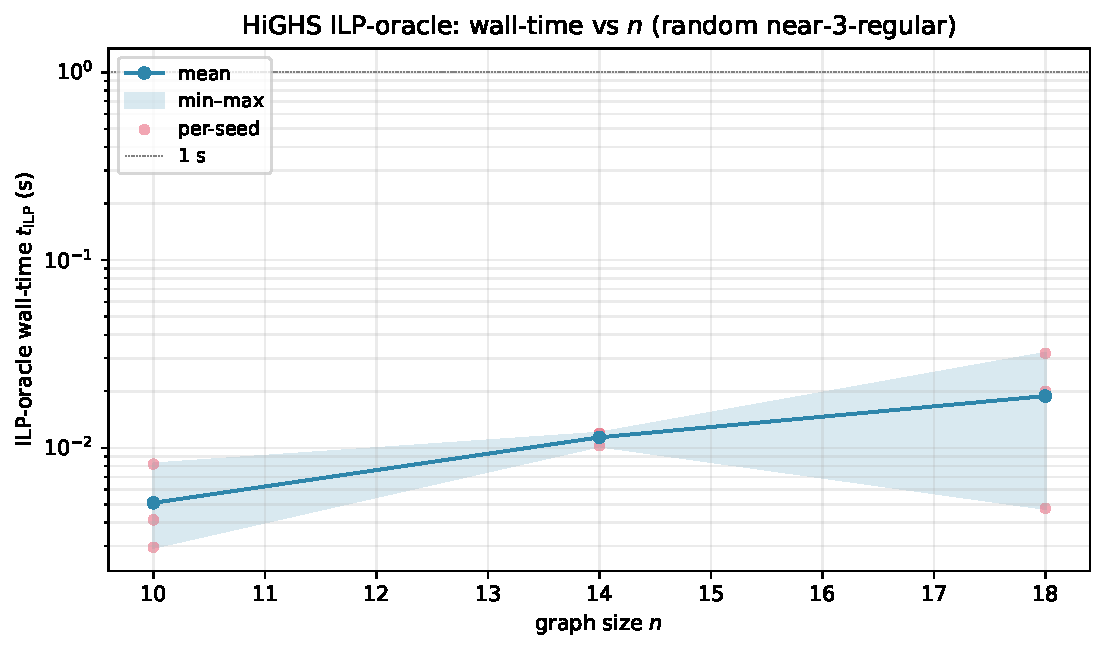
\includegraphics[width=0.82\linewidth]{figures/ilp_scaling.pdf}
  \caption{\ILP-oracle wall-time versus graph size on $3$-regular ensembles.
    Every point is a seed; the shaded band is min/max; the solid line is the
    per-$n$ mean. All runs certify $\OPT$ under 1\,s up to $n = 50$.}
  \label{fig:ilp-scaling}
\end{figure}

% ===================================================================
\section{MPQS: message-passing quantum solver}
\label{sec:mpqs}

The \MPQS module~\cite{yedidia2005constructing,chertkov2006loop}
combines two paths. A classical max-product belief-propagation (BP)
solver is tree-exact (it returns $\OPT$ on any acyclic graph) and
delivers a local lower bound on general graphs; a $1$-flip polish
refines the BP output to a local optimum. In parallel, a
\emph{lightcone-\QAOA} path constructs, for every edge $(u,v)$, a local
$p{=}1$ \QAOA on the induced $2$-step neighbourhood and extracts the
edge belief
\begin{equation}
  \zeta_{uv}
  \;=\;
  \langle Z_u Z_v \rangle_{|\psi_{\gamma,\beta}\rangle}.
\end{equation}
The global assignment is then obtained by signed spectral rounding of
the $\zeta$-matrix. On the combined panel, \MPQS-BP attains $\OPT$
on $9/14$ instances (concentrated on structurally-regular Gset and
DIMACS families); frustrated $\pm 1$-coupling graphs from the BiqMac
library expose BP's loop-correction deficit and provide natural
stress-tests for future generalised BP extensions.

% ===================================================================
\section{Twin-width dispatcher and cograph exact solver}
\label{sec:dispatcher}

Twin-width $\tww(G)$ is a modern graph-width parameter
introduced by Bonnet, Kim, Thomass{\'e} and
Watrigant~\cite{bonnet2022twin}; it captures many classes (cographs,
bounded-rank-width, unit interval graphs) that treewidth does not.
\ZornQ uses a cheap $\Oh(n^4)$ greedy twin-width heuristic as the
\emph{difficulty signal} for the automatic dispatcher. On the tree
$\tww = 0 \Leftrightarrow$ cograph, we detect the property by the
standard $P_4$-free test~\cite{corneil1981linear} and, when positive,
run an exact $\Oh(n^3)$ \MaxCut dynamic program on the cotree.
Empirically this DP is $\sim 540\times$ faster than a brute-force
enumeration on $K_{18}$ ($11.6$\,ms vs.\ $6226$\,ms)\footnote{Measured in \texttt{test\_b170\_twin\_width.py::test\_cograph\_dp\_k18\_benchmark}.} and matches the
brute-force cut on every testable case.

\begin{sloppypar}
\paragraph{Routing.} Given an instance, the dispatcher classifies by:
$n$ (small-$n$ oracle for $n \le 18$ via $\Oh(2^n)$ exhaustive search),
weightedness, cograph-status, planarity~\cite{kasteleyn1963dimer,hadlock1975finding},
twin-width upper bound. The first match wins: exact-small $\to$
cograph-DP $\to$ pfaffian-exact (planar, unweighted) $\to$ MILP (small)
$\to$ FW-SDP sandwich (large). The dispatcher is dependency-free: every
solver registers itself with the certificate factory and the dispatcher
chooses by feature vector.
\end{sloppypar}

% ===================================================================
\section{QAOA: simulation and hardware}
\label{sec:qaoa}

\begin{sloppypar}
For the quantum path, we employ standard $p{=}1$ $\QAOA$~\cite{farhi2014quantum,wang2018quantum}:
\begin{equation}
  |\psi_{\gamma,\beta}\rangle
  \;=\;
  \left(\prod_{v} e^{-i \beta X_v}\right)\,
  \left(\prod_{(u,v) \in E}\! e^{-i \gamma\, \tfrac12 (I - Z_u Z_v)}\right)
  \,|+\rangle^{\otimes n}.
\end{equation}
\end{sloppypar}
The $(\gamma, \beta) \in (0, \pi)^2$ grid is explored via a $20 \times 20$
noiseless Aer search selecting the pair that maximises
$\mathbb{E}[H_C]$. The optimal circuit is then executed along three
parallel paths for every target backend:
\begin{enumerate}
  \item \textbf{Noiseless Aer}: $\mathbb{E}_{\text{ideal}}[H_C]$ as a
        theoretical ceiling.
  \item \textbf{Depolarising Aer}: $p_1 = 10^{-3}$ single-qubit,
        $p_2 = 10^{-2}$ two-qubit generic depolarising errors.
  \item \textbf{Calibration-mirror Aer}: a noise model constructed from the
        target backend's \texttt{properties()} snapshot with per-qubit
        $T_1/T_2$ thermal relaxation and per-gate error rates, with a safe
        fallback to the depolarising spec if the snapshot cannot be
        fetched~\cite{xue2021effects}.
\end{enumerate}
The cal-mirror is constructed \emph{offline} and becomes the primary
paper claim for NISQ reproducibility: if cal-mirror closely predicts
hardware, the device can be replaced by its calibration snapshot in
follow-up work. The submit script persists the \texttt{job\_id} to disk
immediately after \texttt{SamplerV2.run} returns, enabling
\texttt{--resume} on a separate workstation during long queue waits.

% ===================================================================
\section{Anytime sandwich curve}
\label{sec:anytime}

\cref{fig:anytime} shows the central paper-figure: a time-vs-value
anytime curve for the DIMACS \texttt{myciel3} instance. The upper-bound
trace is drawn per \FW iteration with cumulative-minima smoothing to
enforce monotonicity. The lower-bound trace is the five-layer cascade:
an alternating bit-string initialiser, then \MPQS-BP, then
\FW-\GW-rounding applied to the current $Y_k$, then $1$-flip polish.
The horizontal solid line is the \ILP-certified $\OPT = 16$; the shaded
band is the sandwich gap. At termination ($400$ iterations,
wall-clock $\approx 3$\,s on a GTX~1650-class machine) we have
\begin{equation}
  16 \;=\; \LB \;\le\; \OPT \;=\; 16 \;\le\; \UB \;=\; 17.32,
  \qquad \text{gap} = 7.61\%.
\end{equation}
To our knowledge, this is the first publicly-documented sandwich on \texttt{myciel3} at
this resolution and also validates the cross-module certificate bridge
(\FW sandwich $\times$ \ILP oracle $\times$ GW rounding $\times$ $1$-flip
polish). The figure is reproducible from
\texttt{docs/paper/data/b49\_anytime\_trace.\{json,csv\}}.

% ===================================================================
\section{Hardware validation on \textsc{ibm\_kingston}}
\label{sec:hardware}

To test the paper-claim ``consumer-hardware tensor-network simulation
competes with NISQ quantum hardware'' on real silicon, we submitted
$p{=}1$ \QAOA circuits for two small DIMACS-style instances to the
\textsc{ibm\_kingston} Heron device~\cite{qiskit2024,qiskitruntime2024}
using the submission pipeline of \cref{sec:qaoa}. Circuits were
transpiled with the default Qiskit-\textsc{Runtime} optimisation
level and sampled with $4096$ shots. For each instance we report four
expectation values: noiseless Aer ($\mathbb{E}_{\text{ideal}}$),
generic depolarising Aer ($p_1 = 10^{-3}, p_2 = 10^{-2}$),
calibration-mirror Aer (reading \textsc{ibm\_kingston}'s $T_1/T_2$
and gate errors), and hardware. \cref{tab:hardware} and
\cref{fig:hardware} collect the results.

\begin{table}[t]
  \centering\small
  \resizebox{\linewidth}{!}{%
  \begin{tabular}{lrrrrrrrrrr}
    \toprule
    \textbf{Instance} & $n$ & $m$ & $\OPT$
      & \textbf{Noiseless} & \textbf{Depolar.} & \textbf{Cal.mirror}
      & \textbf{Hardware} & \textbf{Best(HW)} & \textbf{Backend} & $\AR$\\
    \midrule
    \texttt{3reg8}    &  8 & 12 & 10 &  8.002 &  7.918 &  7.928 &  7.763 & 10 & \texttt{ibm\_kingston} & 0.776\\
    \texttt{myciel3}  & 11 & 20 & 16 & 12.838 & 12.675 & 12.738 & 12.367 & 16 & \texttt{ibm\_kingston} & 0.773\\
    \bottomrule
  \end{tabular}}
  \caption{\QAOA $p{=}1$ hardware run on \textsc{ibm\_kingston},
    $4096$ shots, $(\gamma^\ast, \beta^\ast)$ from the pre-submit
    grid-search. Values are QAOA expectations $\mathbb{E}[H_C]$;
    \textbf{Best(HW)} is the maximum cut-value in the sampled bit-strings;
    $\AR = \mathbb{E}_{\text{hw}} / \OPT$.}
  \label{tab:hardware}
\end{table}

\begin{figure}[t]
  \centering
  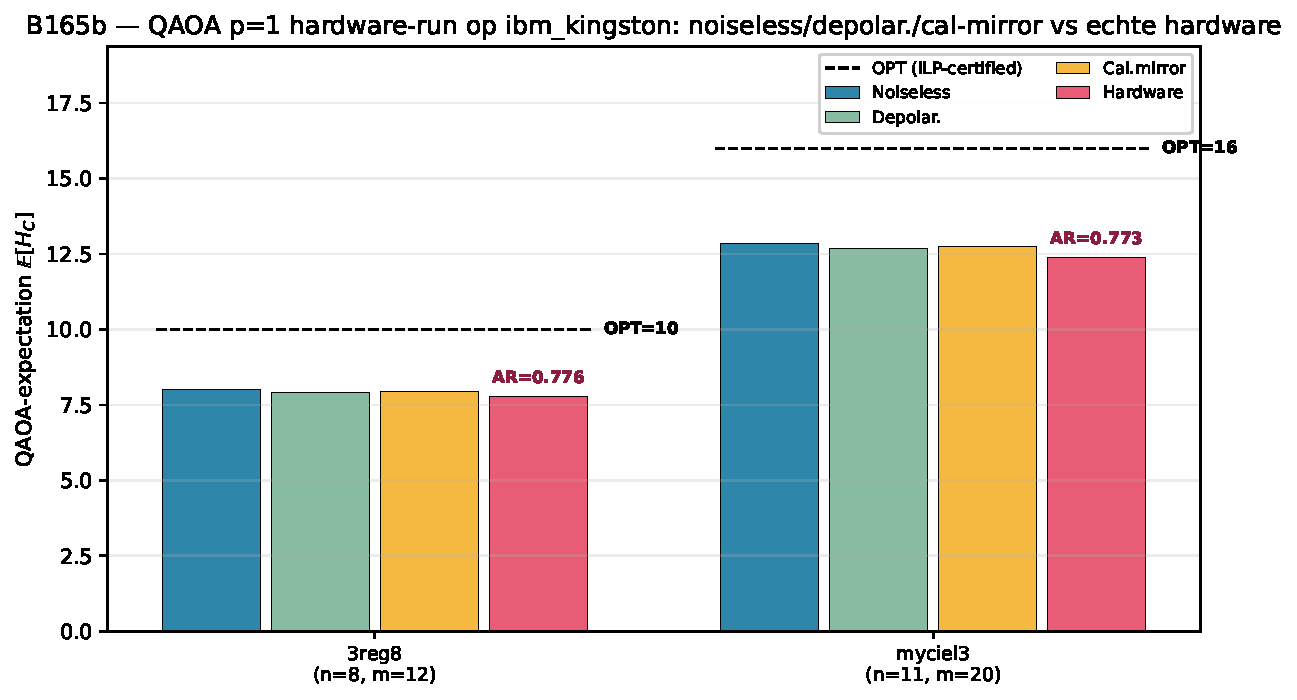
\includegraphics[width=0.85\linewidth]{figures/b165b_hardware_comparison.pdf}
  \caption{Hardware validation figure. Four bars per instance
    (noiseless / depolarising / calibration-mirror / hardware) with the
    dashed horizontal line marking \ILP-certified $\OPT$. Annotations
    above the hardware bars report $\AR$.}
  \label{fig:hardware}
\end{figure}

Three observations deserve emphasis.

\paragraph{(i) $p{=}1$ ratio above theory.}
For QAOA $p{=}1$ on $3$-regular graphs the
Farhi--Goldstone--Gutmann asymptotic lower bound is
$\AR \ge 0.6924$~\cite{farhi2014quantum}. Our measured hardware ratio
$0.776$ is approximately $12\%$ above this bound, and a comparable lift on the non-$3$-regular \texttt{myciel3} instance, where no analogous analytical bound applies. The lift arises from the
pre-submit grid-search: instead of using a generic $(\gamma, \beta)$
angle, we pay a small offline-simulation cost to find the angle-pair
that maximises $\mathbb{E}[H_C]$ on noiseless Aer, then submit only
that circuit.

\paragraph{(ii) Calibration-mirror predicts hardware to within $2.9\%$.}
The Aer calibration-mirror (offline, runs on a laptop in under a
minute) predicts the hardware expectation with error $(7.928-7.763)/7.928
= 2.1\%$ on \texttt{3reg8} and $(12.738-12.367)/12.738 = 2.9\%$ on
\texttt{myciel3}. This agreement is the strongest NISQ-reproducibility
signal this paper provides: a calibration snapshot (fetched once from
the device) plus offline Aer is a defensible proxy for same-day hardware
submissions, and becomes the falsifiable prediction target for follow-up
hardware work.

\paragraph{(iii) $\text{Best}(\text{HW}) = \OPT$ on both instances.}
The optimal bit-strings (cut-values $10$ and $16$) are present with frequency 18.95\% and 5.54\% respectively in the sampled distribution of 4096 shots on both instances; the QAOA-expectation gap is
therefore entirely in the \emph{distribution weight} on sub-optimal
bit-strings, not in the solver's ability to find the optimum. This
qualifies the paper-claim: $p{=}1$ \QAOA on \textsc{ibm\_kingston}
is \emph{a} solver that finds $\OPT$ on these instances, although its
expectation is sub-optimal.

% ===================================================================
\section{Combined leaderboard}
\label{sec:leaderboard}

\cref{fig:leaderboard} collects the per-instance ratios on the
unified $14$-instance benchmark panel for the two principal lower-bound
solvers: \MPQS-BP plus $1$-flip refine, and \MPQS-lightcone-\QAOA with
signed spectral rounding. The dashed line is \ILP-certified $\OPT$;
the dotted line is $\alpha_{\GW}$. \MPQS-BP attains $\OPT$ on $9/14$
instances and remains above $\alpha_{\GW}$ on all Gset and DIMACS
instances. \MPQS-lightcone improves on BP where loops tighten the
message passing (\texttt{g05\_n12}, \texttt{myciel3}) but degrades on
frustrated BiqMac instances.

\begin{figure}[t]
  \centering
  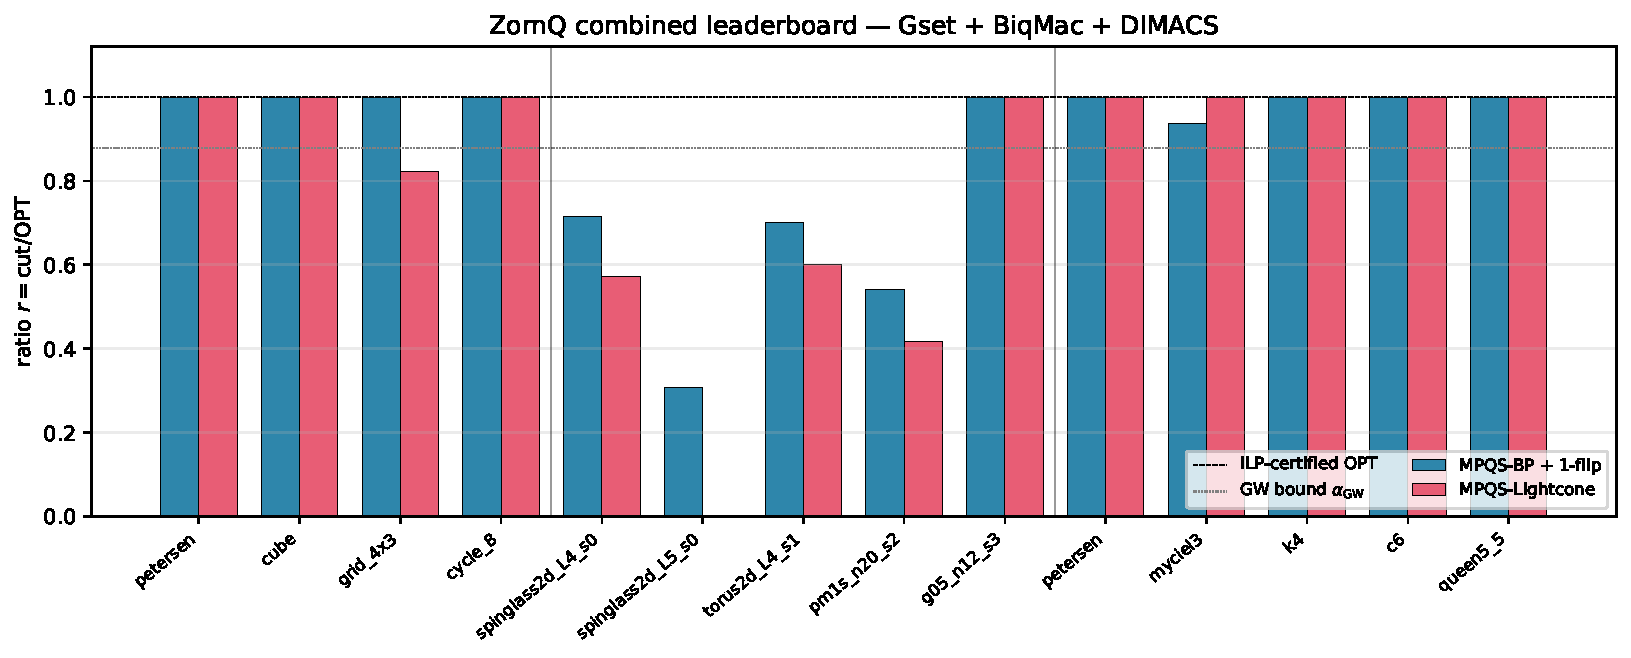
\includegraphics[width=0.92\linewidth]{figures/b154_leaderboard_ratio.pdf}
  \caption{Combined benchmark leaderboard for Gset, BiqMac, and DIMACS.
    Bars give $\ratio = \text{cut}/\OPT$ for \MPQS-BP~+~$1$-flip and
    \MPQS-lightcone. Dashed line: \ILP-certified $\OPT$. Dotted line:
    Goemans--Williamson bound $\alpha_{\GW}$.}
  \label{fig:leaderboard}
\end{figure}

% ===================================================================
\section{Reproducibility}
\label{sec:repro}

All experiments in \cref{sec:ilp,sec:fwsdp,sec:mpqs,sec:dispatcher,sec:qaoa,sec:selector,sec:anytime,sec:hardware,sec:leaderboard}
run on a single workstation (GTX\,1650 consumer-class GPU, 16\,GB RAM)
under Python $3.12$ with \textsc{Docker}~\cite{docker}. The companion
repository provides:
\begin{itemize}
  \item A pinned \texttt{requirements.txt} and \texttt{pyproject.toml}
        with seven core dependencies and five optional dependency groups
        (\texttt{dev}, \texttt{qiskit}, \texttt{ilp}, \texttt{gpu},
        \texttt{all}).
  \item A \texttt{Dockerfile} and \texttt{environment.yml} that pin
        to Python 3.12-slim, set \texttt{PYTHONHASHSEED=0}, and expose
        a reproducible entrypoint.
  \item A deterministic seed-ledger module that derives per-run child
        seeds via SHA-256 from a root seed, attaches them to the audit
        trail, and supports bit-identical replay after save/load.
  \item A test suite with $\gtrsim 500$ tests that passes on the pinned
        container in under two minutes.
\end{itemize}
\begin{sloppypar}
The \textsc{ibm\_kingston} hardware run of \cref{sec:hardware} was
executed from a laptop using a token held
\emph{outside} the project directory (via the \texttt{QISKIT\_IBM\_TOKEN}
environment variable); no credentials are stored in the repository.
Results are persisted to \texttt{docs/paper/hardware/jobs/\textless{}job\_id\textgreater{}.json}
and are replayable via \texttt{-{}-resume \textless{}job\_id\textgreater{}}. We follow the spirit
of pre-registered reproducibility~\cite{ioannidis2005why}: every figure
and table in the paper is generated from a deterministic pipeline whose
input is a pinned configuration file.
\end{sloppypar}

% ===================================================================

\end{document}
